\renewcommand{\chaptername}{Chapter}
\chapter{Realisation}
\label{chap:realisation}
\vspace{-1cm}

\section{Introduction}

This chapter presents the implementation details of One Place Chat, covering the technologies used, frontend and backend architecture, and the key features that make the system unique. We demonstrate how the theoretical concepts discussed in previous chapters translate into a working application.

\section{Tools and Technologies Used}

\subsection{Frontend Technologies}

\vspace{0.8em}
\noindent
\begin{minipage}{0.1\textwidth}
    \includegraphics[height=3em]{LOGOS/React-icon.svg.png}
\end{minipage}%
\begin{minipage}{0.9\textwidth}
    \textbf{Next.js 14 / React 18} \\
    React-based framework providing server-side rendering, file-based routing, and optimized production builds. Used for building the entire user interface including chat components, sidebar navigation, and tools management panel.
\end{minipage}

\vspace{0.8em}
\noindent
\begin{minipage}{0.1\textwidth}
    \includegraphics[height=3em]{LOGOS/Tailwind CSS.png}
\end{minipage}%
\begin{minipage}{0.9\textwidth}
    \textbf{Tailwind CSS} \\
    Utility-first CSS framework enabling rapid UI development with responsive design. Combined with shadcn/ui component library for accessible, customizable interface elements.
\end{minipage}

\vspace{0.8em}
\noindent
\begin{minipage}{0.1\textwidth}
    \includegraphics[height=3em]{LOGOS/download.png}
\end{minipage}%
\begin{minipage}{0.9\textwidth}
    \textbf{TypeScript} \\
    Statically-typed JavaScript providing type safety, enhanced IDE support, and improved code maintainability across both frontend and backend codebases.
\end{minipage}

\subsection{Backend Technologies}

\vspace{0.8em}
\noindent
\begin{minipage}{0.1\textwidth}
    \includegraphics[height=3em]{LOGOS/express-js.png}
\end{minipage}%
\begin{minipage}{0.9\textwidth}
    \textbf{Express.js} \\
    Minimalist web framework for building RESTful APIs with middleware support. Handles all HTTP requests, routing, and API endpoint management.
\end{minipage}

\vspace{0.8em}
\noindent
\begin{minipage}{0.1\textwidth}
    \includegraphics[height=3em]{LOGOS/Gemini.png}
\end{minipage}%
\begin{minipage}{0.9\textwidth}
    \textbf{OpenAI API} \\
    Integration with OpenAI's GPT models for natural language understanding and the \texttt{text-embedding-ada-002} model for generating 1536-dimensional semantic embeddings used in tool matching.
\end{minipage}

\subsection{Database and Storage}

\vspace{0.8em}
\noindent
\begin{minipage}{0.1\textwidth}
    \includegraphics[height=2.5em]{LOGOS/chromadb-no-Text.png}
\end{minipage}%
\begin{minipage}{0.9\textwidth}
    \textbf{ChromaDB} \\
    Open-source vector database designed for AI applications. Stores all application data including tools, conversations, and messages with vector embeddings for semantic similarity search.
\end{minipage}

\subsection{Development Tools}

\vspace{0.8em}
\noindent
\begin{minipage}{0.1\textwidth}
    \includegraphics[height=3em]{LOGOS/github.png}
\end{minipage}%
\begin{minipage}{0.9\textwidth}
    \textbf{Git / GitHub} \\
    Version control and collaboration platform for source code management, feature branching, and code review workflows.
\end{minipage}

\vspace{0.8em}
\noindent
\begin{minipage}{0.1\textwidth}
    \includegraphics[height=3em]{LOGOS/postman-icon.png}
\end{minipage}%
\begin{minipage}{0.9\textwidth}
    \textbf{Postman} \\
    API development and testing platform used for testing backend endpoints, validating request/response structures, and debugging API integrations.
\end{minipage}

\section{Frontend Architecture}

\subsection{Component Hierarchy}

\begin{figure}[H]
    \centering
    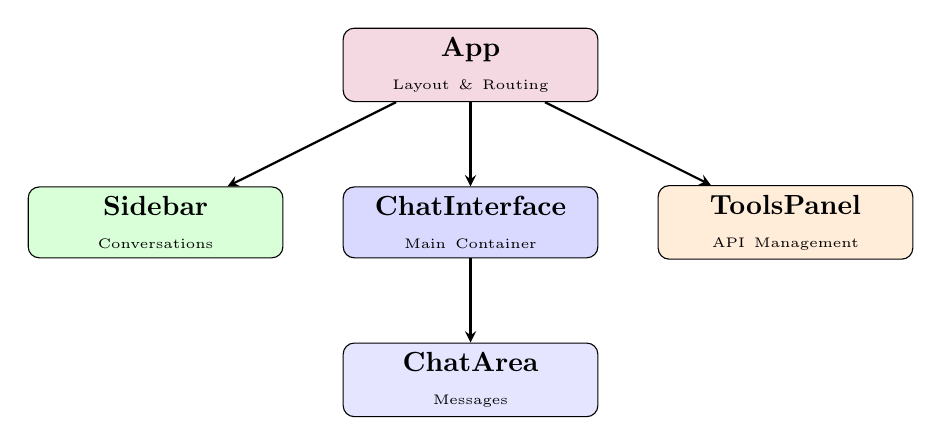
\begin{tikzpicture}[
        node distance=1.5cm,
        box/.style={rectangle, draw, fill=blue!10, text width=3cm, align=center, minimum height=0.8cm, rounded corners},
        arrow/.style={->, >=stealth, thick}
    ]
        \node[box, fill=purple!15] (app) at (0,0) {\textbf{App}\\{\tiny Layout \& Routing}};
        \node[box, fill=green!15] (sidebar) at (-4,-2) {\textbf{Sidebar}\\{\tiny Conversations}};
        \node[box, fill=blue!15] (chat) at (0,-2) {\textbf{ChatInterface}\\{\tiny Main Container}};
        \node[box, fill=orange!15] (tools) at (4,-2) {\textbf{ToolsPanel}\\{\tiny API Management}};
        \node[box] (chatarea) at (0,-4) {\textbf{ChatArea}\\{\tiny Messages}};
        
        \draw[arrow] (app) -- (sidebar);
        \draw[arrow] (app) -- (chat);
        \draw[arrow] (app) -- (tools);
        \draw[arrow] (chat) -- (chatarea);
    \end{tikzpicture}
    \caption{Frontend Component Hierarchy}
    \label{fig:frontend-hierarchy}
\end{figure}

\subsection{Key Components}

\textbf{Sidebar:} Manages conversation navigation, displaying previous sessions with titles and timestamps, and providing new conversation creation.

\textbf{ChatInterface:} Main container orchestrating conversation state, API communication, and real-time message streaming between components.

\textbf{ChatArea:} Renders message bubbles with role-based styling, displays tool execution results, and handles clarification requests with markdown support.

\textbf{ToolsPanel:} Provides OpenAPI specification upload, displays available tools with metadata (method, path, parameters), and manages tool refresh operations.

\section{Backend Architecture}

\subsection{Core Engine Workflow}

\vspace{-0.5cm}
\begin{figure}[H]
    \centering
    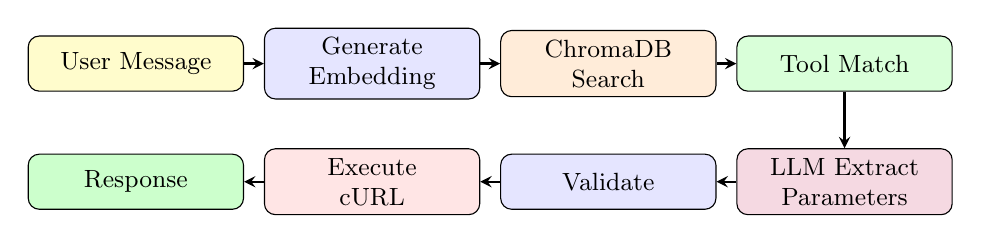
\begin{tikzpicture}[
        node distance=1.2cm,
        box/.style={rectangle, draw, fill=blue!10, text width=2.5cm, align=center, minimum height=0.7cm, rounded corners, font=\small},
        arrow/.style={->, >=stealth, thick}
    ]
        \node[box, fill=yellow!20] (input) at (0,0) {User Message};
        \node[box] (embed) at (3,0) {Generate\\Embedding};
        \node[box, fill=orange!15] (search) at (6,0) {ChromaDB\\Search};
        \node[box, fill=green!15] (match) at (9,0) {Tool Match};
        
        \node[box, fill=purple!15] (extract) at (9,-1.5) {LLM Extract\\Parameters};
        \node[box] (validate) at (6,-1.5) {Validate};
        \node[box, fill=red!10] (execute) at (3,-1.5) {Execute\\cURL};
        \node[box, fill=green!20] (response) at (0,-1.5) {Response};
        
        \draw[arrow] (input) -- (embed);
        \draw[arrow] (embed) -- (search);
        \draw[arrow] (search) -- (match);
        \draw[arrow] (match) -- (extract);
        \draw[arrow] (extract) -- (validate);
        \draw[arrow] (validate) -- (execute);
        \draw[arrow] (execute) -- (response);
    \end{tikzpicture}
    \caption{Backend Request Processing Flow}
    \label{fig:backend-flow}
\end{figure}

\textbf{OpenAPI Parsing:} Converts API specs into executable MCPTool objects with paths, methods, and schemas.

\textbf{Semantic Matching:} Generates embeddings via OpenAI, performs similarity search in ChromaDB, returns ranked matches.

\textbf{LLM Extraction:} Extracts structured parameters from natural language using GPT, validates and requests clarification if needed.

\textbf{API Execution:} Generates and executes cURL commands, formats responses for display.


\section{Application Interfaces}

\subsection{Main Chat Interface}

\begin{figure}[H]
    \centering
    \setlength{\fboxrule}{1pt}
    \setlength{\fboxsep}{0pt}
    \fbox{\includegraphics[width=0.95\linewidth]{screens/chat-app-interface.png}}
    \caption{One Place Chat Main Interface}
    \label{fig:chat-interface}
\end{figure}

Key features of the main interface:
\begin{itemize}
    \item \textbf{Sidebar}: Displays conversation history with timestamps and quick access to previous sessions
    \item \textbf{Chat Area}: Central message display with role-based styling for user and assistant messages
    \item \textbf{Tools Panel}: Shows available API tools loaded from OpenAPI specifications
    \item \textbf{Input Field}: Natural language input for API requests
\end{itemize}

\subsection{Chat Message Response}

The system displays API responses in a formatted, user-friendly manner:

\begin{figure}[H]
    \centering
    \setlength{\fboxrule}{1pt}
    \setlength{\fboxsep}{0pt}
    \fbox{\includegraphics[width=1\linewidth]{screens/chat-message response.png}}
    \caption{Chat Message Response Display}
    \label{fig:chat-response}
\end{figure}

Response features include:
\begin{itemize}
    \item Formatted JSON output for API responses
    \item Markdown rendering for rich text formatting
    \item cURL command display for transparency
    \item Error handling with helpful messages
\end{itemize}
\newpage
\subsection{Tool Description Panel}

When a user selects a tool, the panel displays its complete specification including the tool name, HTTP method badge, endpoint path, and a description of its functionality. The parameters section lists all required and optional fields with their types, helping users understand what information is needed.

\begin{figure}[H]
    \centering
    \setlength{\fboxrule}{1pt}
    \setlength{\fboxsep}{0pt}
    \fbox{\includegraphics[width=0.6\linewidth]{screens/tool-description.png}}
    \caption{Tool Description Panel}
    \label{fig:tool-description}
\end{figure}

The panel content includes:
\begin{itemize}
    \item \textbf{Name}: Tool identifier generated from the API operation
    \item \textbf{Description}: What the tool does and its purpose
    \item \textbf{Endpoint}: Full API path with HTTP method (GET, POST, PUT, DELETE)
    \item \textbf{Arguments}: Required and optional parameters with data types
    \item \textbf{Response}: Expected response format and structure
    \item \textbf{Status}: Tool availability and deprecation warnings
\end{itemize}

\newpage

\subsection{Documentation Upload}

The documentation upload interface allows users to add new API tools:

\begin{figure}[H]
    \centering
    \setlength{\fboxrule}{1pt}
    \setlength{\fboxsep}{0pt}
    \fbox{\includegraphics[width=0.5\linewidth]{screens/documentation-upload.png}}
    \caption{OpenAPI Documentation Upload Interface}
    \label{fig:doc-upload}
\end{figure}

Upload features include:
\begin{itemize}
    \item Drag-and-drop file upload for OpenAPI specifications
    \item Support for JSON and YAML formats
    \item Automatic tool generation from uploaded specs
    \item Visual feedback on upload progress and success
\end{itemize}

\section{Conclusion}

This chapter presented the complete implementation of One Place Chat, from the technology stack to the user interfaces. The frontend, built with Next.js and React, provides an intuitive conversational experience through well-structured components: Sidebar for navigation, ChatInterface for message orchestration, ChatArea for display, and ToolsPanel for API management.



